\section{Data and design}
\label{sec:design}
We define Sybils in the Tor network as two or more relays that are under central
control.  Sybils per se do not have to be malicious; a relay operator could
simply have forgotten to configure the \texttt{MyFamily} option that is used to
express that multiple relays are under central control.  Such Sybils are no
threat to the Tor network, which is why we refer to them as \emph{benign
Sybils}.  What we are interested in is \emph{malicious Sybils} whose purpose is
to deanonymize or otherwise harm Tor users.

We draw on two datasets, one publicly available and one created by us, to
uncover malicious Sybils.  Our detection methods are implemented in a tool,
\sys, which takes as input our two datasets and then attempts to expose Sybil
groups, as illustrated in Figure~\ref{fig:system}.  \Sys is implemented in Go
and consists of 3,300 lines of code.

\begin{figure}[t]
	\centering
	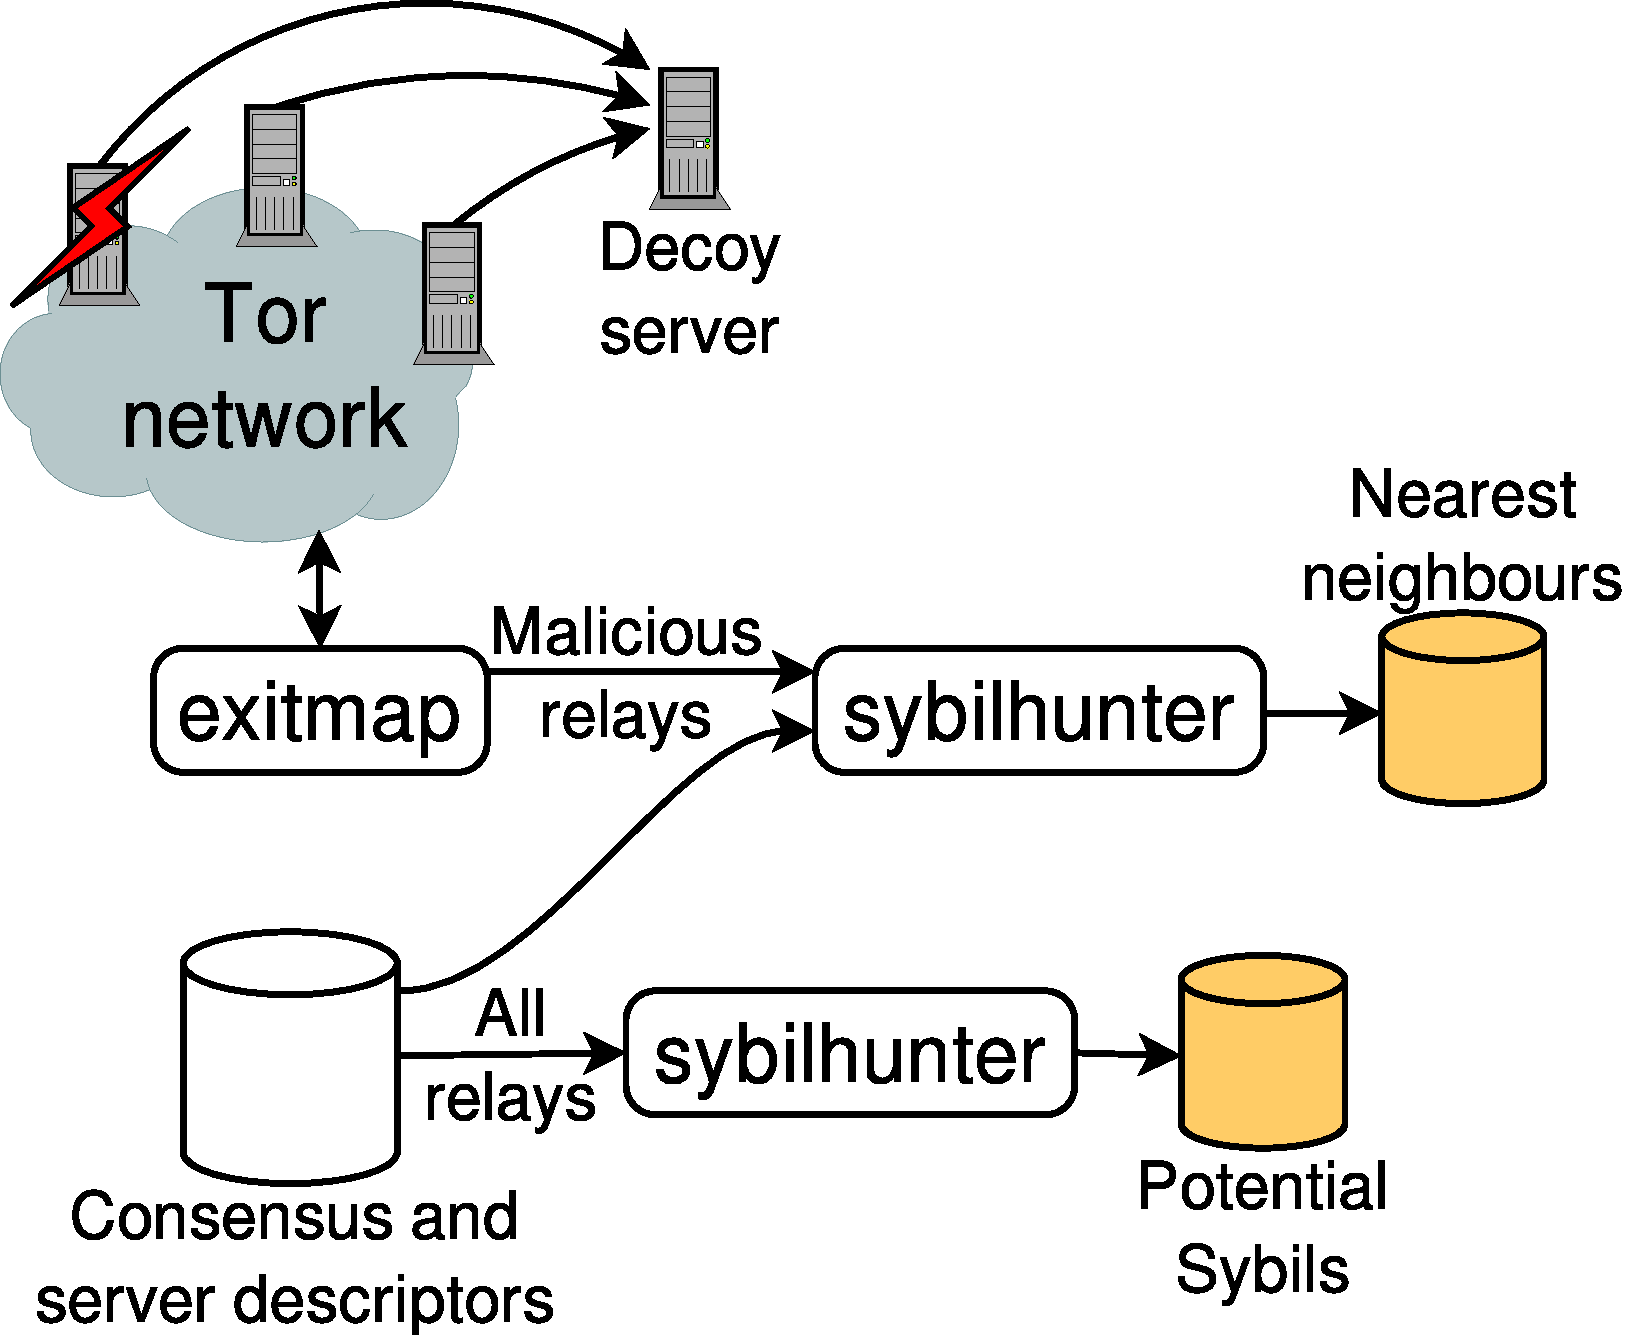
\includegraphics[width=\linewidth]{diagrams/system_architecture.pdf}
	\caption{\Sys's architecture.  Two datasets serve as input to
		\sys; archived consensuses and server descriptors, and malicious
		relays that we gather by running exitmap~\cite{Winter2014a}.}
	\label{fig:system}
\end{figure}

\subsection{Datasets}
\label{sec:datasets}
Figure~\ref{fig:system} shows how we use our two datasets.  Archived consensuses
and router descriptors (in short: descriptors) allow us to (\emph{i}) restore
past states of the Tor network, which \sys mines for Sybil groups, and to
(\emph{ii}) find ``partners in crime'' of malicious exit relays that we
discovered by running exitmap, a scanner for Tor exit relays.

\subsubsection{Consensuses and router descriptors}
The consensus and descriptor dataset is publicly available on
CollecTor~\cite{collector}, a service that is run by The Tor Project and
archives network data such as consensuses, descriptors, and network status
votes.  Some of the archived data dates back to 2004, allowing us to restore
arbitrary Tor network configurations from the last ten years.  Not all of
CollecTor's archived data is relevant to our hunt for Sybils, however, which is
why we only analyse the following two:

\begin{figure}[t]
\centering
\begin{tikzpicture}[node distance=0 cm,outer sep = 0pt,inner sep = 2pt]

	\tikzstyle{every node}=[font=\footnotesize]

	\tikzset{field/.style={align=center,shape=rectangle,
		minimum height=4mm,minimum width=23mm,fill=gray!20}}

	\tikzset{blankfield/.style={align=center,shape=rectangle,
		minimum height=4mm,minimum width=23mm}}

	\usetikzlibrary{positioning}

	\node (consensus) [blankfield] {\textbf{Consensus}};

	% Router status fields, one below another.
	\node (routerstatus) [blankfield,below=of consensus] {\textbf{Router status}};
	\node (desc) [field,below=of routerstatus] {Descriptor pointer};
	\node (nickname) [field,below=of desc] {Nickname};
	\node (fingerprint) [field,below=of nickname] {Fingerprint};
	\node (publication) [field,below=of fingerprint] {Publication};
	\node (address) [field,below=of publication] {Address and ports};
	\node (flags) [field,below=of address] {Flags};
	\node (version) [field,below=of flags] {Version};
	\node (bandwidth) [field,below=of version] {Bandwidth};
	\node (policy) [field,below=of bandwidth] {Exit policy};
	\node [below=of policy] {\textbf{\dots}};

	% Draw a rectangle around a router status.
	\draw [draw=black] (desc.north west) rectangle (policy.south east);

	% Draw a rectangle around multiple router statuses.
	\draw [draw=black] ($(desc.north west) + (-2mm,4.5mm)$) rectangle ($(policy.south east) + (2mm,-4.5mm)$);

	% Router descriptor fields, one below another.
	\node (dummy) at (4cm,0) [blankfield] {};
	\node (descriptor) at (4cm,0) [blankfield,below=of dummy] {\textbf{Router descriptor}};
	\node (descaddr) at (4cm,0) [field,below=of descriptor] {Address and ports};
	\node (descplatform) at (4cm,0) [field,below=of descaddr] {Platform};
	\node (descprotocols) at (4cm,0) [field,below=of descplatform] {Protocols};
	\node (descpublished) at (4cm,0) [field,below=of descprotocols] {Published};
	\node (descfingerprint) at (4cm,0) [field,below=of descpublished] {Fingerprint};
	\node (descuptime) at (4cm,0) [field,below=of descfingerprint] {Uptime};
	\node (descbandwidth) at (4cm,0) [field,below=of descuptime] {Bandwidth};
	\node (descsignature) at (4cm,0) [field,below=of descbandwidth] {Signature};

	% Draw a rectangle around a descriptor.
	\draw [draw=black] (descaddr.north west) rectangle (descsignature.south east);

	% Pointer from digest to descriptor.
	\draw [-latex,thick] (desc) -- (descaddr);
\end{tikzpicture}
\caption{Our primary dataset contains consensuses and router descriptors.}
\label{fig:datasets}
\end{figure}

\paragraph{Descriptors} Tor relays and bridges periodically upload router
descriptors, that capture their configuration, to directory authorities.
Figure~\ref{fig:datasets} shows an example in the box to the right.  Relays
upload their descriptors no later than every 18 hours, or sooner, depending on
certain conditions.  Note that some information in router descriptors is not
verified by directory authorities.  Therefore, relays can spoof information such
as their operating system, Tor version, and uptime.

\paragraph{Consensuses} Each hour, the nine directory authorities vote on their
view of all Tor relays that are currently online.  The vote produces the
consensus, an authoritative list that comprises all running Tor relays,
represented as a set of router statuses.  Each router status in the consensus
contains basic information about Tor relays such as their bandwidth, flags, and
exit policy.  It also contains a pointer to the relay's descriptor, as shown in
Figure~\ref{fig:datasets}.  As of January 2016, consensuses contain approximately
7,000 router statuses, i.e., each hour, 7,000 router statuses are published, and
archived by CollecTor.

Table~\ref{tab:collector-dataset} gives an overview of the size of our consensus
and descriptor archives.  We found it challenging to repeatedly process these
millions of files, amounting to almost 100 GiB of uncompressed data.  In our
first processing attempt, we used the Python parsing library Stem~\cite{stem},
which is maintained by The Tor Project.  The data volume turned out to be
difficult to handle for Stem because of Python's interpreted and dynamic nature.
To process our dataset more efficiently, we implemented a custom parser in Go.
% Our parser has approximately 1,300 lines of code (and 900 additional lines for
% tests) and supports both strict and lazy parsing.  According to our benchmarks,
% our parser can process approximately 27 consensuses per second, as measured on
% an Intel Core i7 2.9 GHz CPU, a consumer-grade CPU.  We placed our datasets on a
% solid state drive to eliminate the I/O bottleneck.  Stem, for comparison,
% averages at around 1.8 consensuses per second.  Note, however, that Stem
% processes more fields than our parser, which makes it difficult to have a fair
% comparison.

\begin{table}[t]
\small
\centering
\begin{tabular}{l c c c}
\textbf{Dataset} & \textbf{\# of files} & \textbf{Size} & \textbf{Time span} \\
\hline
% find . -type f | wc -l
% du -b consensuses/
Consensuses & 72,061 & 51 GiB & 10/2007--01/2016 \\
Descriptors & 34,789,777 & 52 GiB & 12/2005--01/2016 \\
\end{tabular}
\caption{An overview of our primary dataset, consensuses and server descriptors
since 2007 and 2005, respectively.}
\label{tab:collector-dataset}
\end{table}

\subsubsection{Malicious relays}
In addition to our publicly available and primary dataset, we collected
malicious exit relays over 18 months.  We add these relays to our dataset
because they frequently \emph{surface in groups}, as malicious Sybils, because
an attacker runs the same attack on several, physically distinct exit
relays.  Winter et al.'s work~\cite[\S 5.2]{Winter2014a} further showed that
attackers make an effort to stay under the radar, which is why we cannot only
rely on active probing to find such relays.  We also seek to find potential
``partners in crime'' of each newly discovered malicious relay, which we discuss
in Section~\ref{sec:nearest-neighbor}.

We exposed malicious exit relays using Winter et al.'s exitmap tool~\cite[\S
3.1]{Winter2014a}.  Exitmap is a Python-based scanning framework for Tor exit
relays.  Exitmap modules perform a network task that can then be run over all
exit relays.  One use case is HTTPS man-in-the-middle detection: A module can
fetch the certificate of a web server over all exit relays and then compare its
fingerprint with the expected, valid fingerprint.  Exposed attacks, however, can
be difficult to attribute because an attack can take place upstream of the exit
relay, e.g., at a malicious autonomous system.

In addition to the original modules that the exitmap authors shared with us, we
implemented exitmap modules to detect HTML tampering and TLS downgrading, by
connecting to servers under our control and raising an alert if the returned
HTML or TLS server hello were modified.  Our modules ran from Aug 2014 to
January 2016 and discovered 205 malicious exit relays, shown in
Appendix~\ref{sec:malicious-relays}, that we all reported to The Tor Project.

\subsection{Threat model}
\label{sec:threat_model}
Most of our work is on applying \sys on archived data.  We can also apply \sys
on newly incoming data, but that means that adversaries can manipulate
their Sybil configuration to evade our system, and the powerful nature of Sybil
attacks~\cite{Douceur2002a} limits our defenses.  This is reflected in our
adversarial assumptions.

We assume that an adversary \emph{does}:
\begin{itemize}
	\item Run more than one Tor relay.

	\item Exhibit redundancy in their relay configuration, or uptime sequence.
\end{itemize}

An adversary further \emph{can}:
\begin{itemize}
	\item Add Tor relays all at once or slowly over time.

	\item Know about \sys.

	\item Run active or passive attacks.

	\item Make a limited effort to stay under the radar by diversifying parts of
		their configuration.  To detect Sybils, however, our heuristics require
		\emph{some} redundancy.
\end{itemize}

\subsection{Analysis techniques}
\label{sec:techniques}
Having discussed our datasets and threat model, we now turn to presenting
techniques that can expose Sybils.  Our techniques are based on the insight that
Sybil relays typically \emph{behave appear similarly}.  Shared configuration
parameters such as port numbers and nicknames cause similar appearance.  Sybils
behave similarly when they reboot simultaneously and might exhibit the same
quirks when relaying traffic.

\Sys can analyze (\emph{i}) historical network data, dating back to 2007;
(\emph{ii}) online data, to detect new Sybils as they join the network; and
(\emph{iii}) find relays that might be associated with previously discovered,
malicious relays.  Figure~\ref{fig:shr-internal} shows \sys's internal
architecture.  Tor network data first passes a filtering component that can be
used to inspect a subset of the data.  It is then forwarded to one or more
modules that implement an analysis technique.  These modules work independently,
but share a data structure to find suspicious relays that show up in more than
one module.  Depending on the analysis technique, \sys's output is CSV
files or images.

\begin{figure}[t]
	\centering
	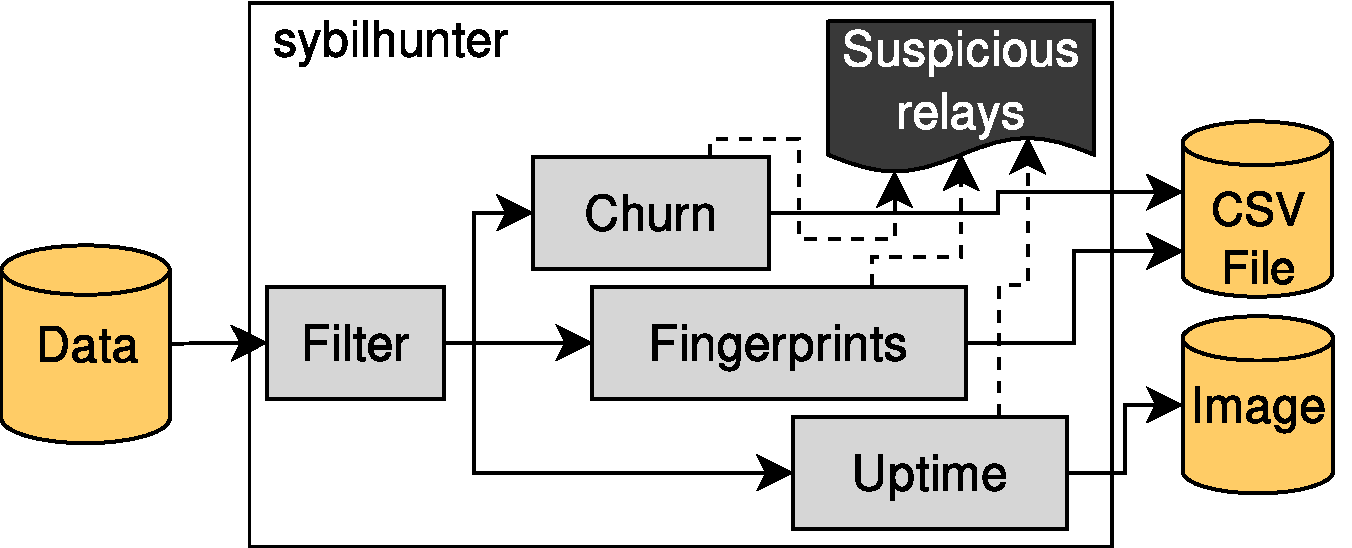
\includegraphics[width=0.9\linewidth]{diagrams/sybilhunter-internal.pdf}
	\caption{\Sys's internal architecture.}
	\label{fig:shr-internal}
\end{figure}

While developing \sys, we had to make many design decisions that we
tackled by drawing on the experience we gained by manually analyzing numerous
Sybil groups.  We iteratively improved our code and augmented it with new
features when we experienced operational shortcomings.

\subsubsection{Network churn time series}
\label{sec:churn-time-series}
The churn rate of a distributed system captures the rate of joining and leaving
network participants.  In the Tor network, these participants are relays.  An
unexpectedly high churn rate between two subsequent consensuses means that many
relays joined or left, which can reveal Sybils and other network issues because
Sybil operators frequently start and stop their Sybils at the same time to ease
administration---they behave similarly.

The Tor Project is maintaining a Python script~\cite{doctor} that determines the
number of previously unobserved relay fingerprints in new consensuses.  If that
number is greater than or equal to the static threshold 50, the script sends an
email alert.  The threshold was chosen arbitrarily.  We reimplemented the script
in \sys and ran it over all archived consensus documents, dating back to
2007.  The script raised 47 alerts in nine years, all of which seemed to be true
positives, i.e., they should be of interest to The Tor Project.  The script did
not raise false positives because the median number of new fingerprints in a
consensus is only six---significantly below the conservative threshold of 50.
Conversely, the threshold likely causes false negatives, but we cannot determine
the false negative rate because we lack ground truth.  In addition, The Tor
Project's script does not consider relays did leave the network and it can be
defeated by a ``trickling'' attack in which Sybils are slowly added over time.
We now extend The Tor Project's approach to make it more robust against these
shortcomings.

We found that churn anomalies worthy of our attention range from \emph{flat
hills} (Fig.~\ref{fig:flat-hill}) to \emph{sudden spikes}
(Fig.~\ref{fig:sudden-spike}).  Flat hills can be a sign of an event that
concerned a large number of relays, over many hours or days.  Such an event
happened shortly after the heartbleed bug, when The Tor Project asked relay
operators to generate new keys.  Relay operators acted gradually, over
approximately two days.  Sudden spikes can happen if an attacker adds many
relays, all at once.

\begin{figure}[t]
	\centering
	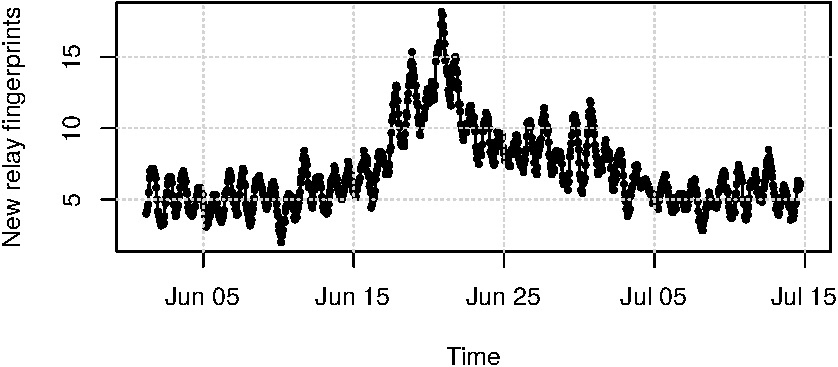
\includegraphics[width=\linewidth]{diagrams/flat-hill.pdf}
	\caption{A flat hill of new relays in 2009.  The time series was smoothed
	using a moving average with a window size of 12 hours.}
	\label{fig:flat-hill}
\end{figure}

\begin{figure}[t]
	\centering
	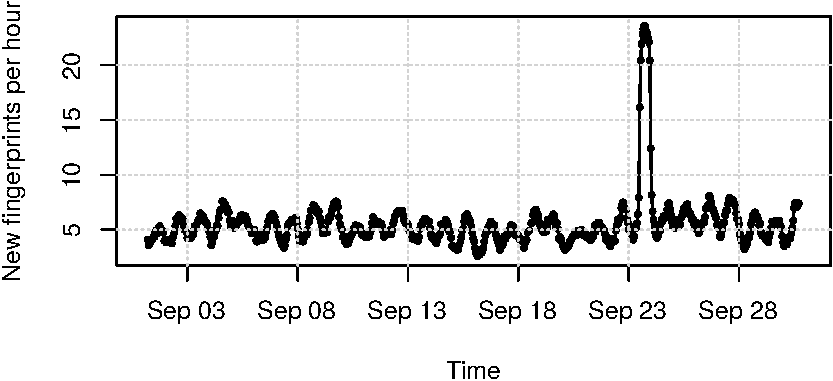
\includegraphics[width=\linewidth]{diagrams/sudden-spike.pdf}
	\caption{A sudden spike of new relays in 2010.  The time series was smoothed
	using a moving average with a window size of 12 hours.}
	\label{fig:sudden-spike}
\end{figure}

To quantify the churn rate $\sigma$ between two subsequent consensus documents,
we adapt Godfrey et al.'s~\cite{Godfrey2006a} formula, which yields a scalar
churn value that captures both systems that joined and systems that left the
network.  An unusually low number of systems that left could cancel out an
unusually high number of new systems---an undesired property for a technique
that should spot abnormal changes.  To address this issue, we split the formula
in two parts, creating a time series for new relays ($\sigma_{n}$) as well as
for relays that left ($\sigma_{g}$).  $C_{t}$ is the network consensus at time
$t$, and $\setminus$ denotes the complement between two consensuses, i.e., the
relays that are in one consensus, but not the other.  We define $\sigma_{n}$ and
$\sigma_{g}$ as

% \begin{figure}[t]
% 	\centering
% 	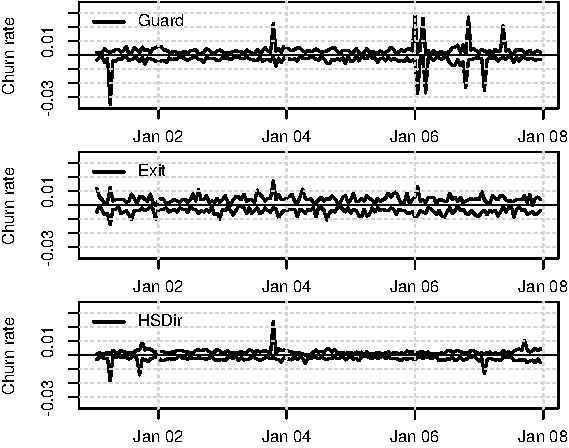
\includegraphics[width=\linewidth]{diagrams/churn-example.pdf}
% 	\caption{Churn time series for the first week of 2016.  The three diagrams
% 		illustrate the churn rate of all relays with the \texttt{Guard},
% 		\texttt{Exit}, and \texttt{HSDir} flag, respectively.}
% 	\label{fig:churn-example}
% \end{figure}

\begin{equation}
\sigma_{n} = \frac{\lvert C_{t} \setminus C_{t-1} \rvert}
%{\textrm{max}\{\lvert C_{t-1} \rvert, \lvert C_{t} \rvert \}}
{\lvert C_{t} \rvert}
\qquad\text{and}\qquad
\sigma_{g} = \frac{\lvert C_{t-1} \setminus C_{t} \rvert}
%{\textrm{max}\{\lvert C_{t-1} \rvert, \lvert C_{t} \rvert \}}
{\lvert C_{t-1} \rvert}.
\end{equation}

Both $\sigma_{n}$ and $\sigma_{g}$ are bounded to the interval $[0, 1]$.  A
churn value of 0 indicates no change between two subsequent consensuses whereas
a churn value of 1 indicates a complete turnover.  Determining $\sigma_{n,g}$
for the sequence $C_{t}, C_{t-1}$, \ldots, $C_{t-n}$, yields a time series of
churn values that can readily be inspected for abnormal spikes.  We found that
many churn anomalies are caused by relays that share a flag, or a flag
combination, e.g., \texttt{HSDir} and \texttt{Exit}.  Therefore, \sys can
also generate per-flag churn time series that can uncover patterns that would be
lost in a universal time series.

Finally, to detect changes in the underlying time series trend---flat hills---we
can smooth $\sigma_{n,g}$ using a simple moving average $\lambda$ defined as

\begin{equation}
\lambda = \frac{1}{w} \cdot \sum_{i=0}^{w} \sigma_{i}
\end{equation}

As we increase the window size $w$, we can detect more subtle changes in the
underlying churn trend.  If $\lambda$ or $\sigma_{n,g}$ exceed a manually
defined threshold, an alert is raised.  Section~\ref{sec:churn} discusses how a
threshold can be chosen.

\subsubsection{Uptime matrix}
\label{sec:uptime-matrix}
For convenience, attackers are likely to administer their Sybil relays
simultaneously, i.e., update, configure, and reboot them all at the same time.
This is reflected in their relays' uptime.  When an attacker installs an
operating system upgrade on her Sybils, we will observe a set of relays going
offline and back online at the same time.  To isolate such events, we are
visualizing the \emph{uptime patterns} of Tor relays by grouping together relays
whose uptime is highly correlated.  The churn technique is similar but it only
provides an aggregate, high-level view on how Tor relays join and leave the
network.  Since the technique is aggregate, it is poorly suited for visualizing
the uptime of specific relays; an abnormally high churn value attracts our
attention but does not tell us what caused the anomaly.  To fill this gap, we
complement the churn analysis with a qualitative technique that visualizes the
uptime of specific relays---an uptime matrix that we will now present.

This uptime matrix consists of the uptime patterns of all Tor relays, which we
represent as binary sequences.  Each hour, when a new consensus is published, we
add a new data point---``online'' or ``offline''---to each Tor relay's sequence.
We visualize all sequences in a bitmap whose rows represent consensuses and
whose columns represent relays.  Each pixel denotes the uptime status of a
particular relay at a particular hour.  Black pixels mean that the relay was
online and white pixels mean that the relay was offline.  This type of
visualization was first proposed by Ensafi and subsequently implemented by
Fifield~\cite{Fifield2014a}.

Of particular importance is how the uptime sequences are sorted.  If highly
correlated sequences are not adjacent in the visualization, we might miss them.
We sort sequences using single-linkage clustering, a type of hierarchical
clustering algorithm that forms groups bottom-up, based on the minimum distance
between group members.  Similar to Andersen et al.~\cite{Andersen2002a}, we use
Pearson's correlation coefficient in our distance function because it tells us
if two uptime sequences change together.  The sample correlation coefficient $r$
% between two vectors $x = (x_1, \cdots, x_n)$ and $y = (y_1, \cdots, y_n)$ is
% defined as
% 
% \begin{equation}
% r = \frac{\sum_{i=1}^{n} (x_{i} - \bar{x}) (y_{i} - \bar{y})}
% {\sqrt{\sum_{i=1}^{n} (x_{i} - \bar{x})^2} \sqrt{\sum_{i=1}^{n} (y_{i} - \bar{y})^2}}
% \end{equation}
% 
yields a value in the interval $[-1, 1]$.
%The sample mean is given by
%$\bar{x}$ and $\bar{y}$.
A coefficient of $-1$ denotes perfect anti-correlation
(relay $R_1$ is only online when relay $R_2$ is offline) and 1 denotes perfect
correlation (relay $R_1$ is only online when relay $R_2$ is online).  We define
our distance function as $d(r) = 1 - r$, so two perfectly correlated sequences
have a distance of zero while two perfectly anti-correlated sequences have a
distance of two.  Once all sequences are sorted, we color adjacent sequences in
red if their uptime sequence is identical.  Figure~\ref{fig:uptime-matrix} shows
an example of our visualization algorithm, the uptime matrix for a subset of all
Tor relays in Nov 2012.

\begin{figure}[t]
	\centering
	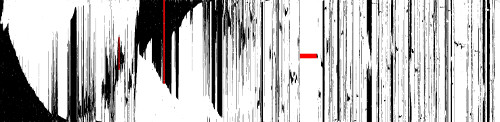
\includegraphics[width=\linewidth]{diagrams/2012-11.jpg}
	\caption{The uptime matrix for a subset of all Tor relays in Nov 2012.}
	\label{fig:uptime-matrix}
\end{figure}

\subsubsection{Fingerprint analysis}
\label{sec:fingerprint-analysis}
The information a Tor client needs to connect to an onion service is stored in a
DHT that consists of a subset of all Tor relays, the onion service directories
(HSDirs).  As of January 2016, 42\% of all Tor relays serve as HSDir.  A
daily-changing set of six HSDirs host the contact information of any given
onion service.  Tor clients contact one of these six HSDirs to request
information about the onion service they intend to connect to.  A HSDir becomes
responsible for an onion service if the difference between its relay fingerprint
and the service's descriptor ID is small.  The descriptor ID is derived from the
onion service's public key, a time stamp, and additional information.
% https://gitweb.torproject.org/torspec.git/tree/rend-spec.txt:231
% descriptor-id = H(permanent-id | H(time-period | descriptor-cookie | replica))
All HSDirs are public, making it possible to determine at which position in the
DHT an onion service will end up at any point in the future.  Attackers can
exploit the ability to predict the DHT position by repeatedly generating
identity keys until their fingerprint is sufficiently close to the targeted
onion service's index, thus becoming its HSDir~\cite{Biryukov2013a}.

We detect relays that change their fingerprint frequently by maintaining a
lookup table that maps a relay's IP addresses to a list of all fingerprints we
have seen it use.  We sort the lookup table by the relays that changed their
fingerprints the most, and output the results.

\subsubsection{Nearest-neighbor search}
\label{sec:nearest-neighbor}
We frequently found ourselves in a situation where exitmap discovered a
malicious exit relay and we were left wondering if there were similar,
potentially associated relays.  Looking for such relays involved extensive
manual work, which we soon started to automate.  We needed an algorithm for
nearest-neighbor search that takes as input a ``seed'' relay and finds its $n$
most similar neighbors.  We define similarity as shared configuration parameters
such as port number, IP addresses, exit policies, or bandwidth.  Our search
algorithm sorts relays by comparing these configuration parameters.

To quantify the similarity between two relays, we use the Levenshtein distance,
a popular distance metric that takes as input two strings and determines the
minimum number of modifications---insert, delete, and modify---that are
necessary to turn string $s_{1}$ into $s_{2}$.  Our algorithm extracts several
configuration parameters of two relays, turns them into strings, and determines
their Levenshtein distance.  As an example, consider a simplified configuration
representation consisting of the concatenation of nickname, IP address, and
port.  To turn the string $s_2$ into $s_1$, six operations are necessary; three
modifications (green) and two deletions (red):

\definecolor{change}{rgb}{0.7,1.0,0.7}
\definecolor{delete}{rgb}{1.0,0.7,0.7}

$s_1$: \texttt{Foo10.0.0.19001}

$s_2$: \texttt{\setlength{\fboxsep}{0pt}%
\colorbox{change}{\strut Bar}10.0.0.%
\colorbox{change}{\strut 2}%
\colorbox{delete}{\strut 54}%
9001}

We implemented a simple linear search to determine the Levenshtein distance
between a given relay and all other relays that are part of the same consensus.
For a consensus consisting of 6,525 relays, our algorithm takes approximately
1.5 seconds to finish.\footnote{We measured on an Intel Core i7-3520M CPU at 2.9
GHz, a consumer-grade CPU.}

\subsubsection{Narrowing the semantic gap}
Systems that employ complex and opaque analysis techniques frequently suffer
from what Sommer and Paxson call the \emph{semantic gap}~\cite[\S
III.C]{Sommer2010a}, a gap in understanding what a system's output means and how
it should be acted upon.  Our techniques automate the \emph{detection} of
Sybils, but the process of \emph{blocking} them involves human interaction.  If
The Tor Project must spend hours to understand and verify \sys alerts,
our techniques are ultimately useless.  Therefore, we took special care to
narrow the semantic gap.

We avoid the use of opaque classification methods because their
output---frequently distances in high-dimensional vector space---is difficult to
interpret.  Instead, we use the Levenshtein distance because its output is easy
to understand and retrace.  Finally, in accordance with the Unix tool design
philosophy~\cite{Pike1983a}, \sys produces CSV-formatted text output that
is easy to pipe into command line tools such as cut, grep, and awk for further
analysis.
